\documentclass[conference]{IEEEtran}
\IEEEoverridecommandlockouts

\usepackage{mathptmx}
\usepackage{graphicx}
\usepackage{booktabs}
\usepackage{multirow}
\usepackage{amsmath}
\usepackage{amssymb}
\usepackage{subcaption}
\usepackage{hyperref}
\usepackage{xcolor}

\hypersetup{
    colorlinks=true,
    linkcolor=black,
    citecolor=black,
    urlcolor=blue,
}

\def\BibTeX{{\rm B\kern-.05em{\sc i\kern-.025em b}\kern-.08em
    T\kern-.1667em\lower.7ex\hbox{E}\kern-.125emX}}

\begin{document}

\title{\fontfamily{ptm}\selectfont LLM Inference Latency Using Prompt-Aware Learning-to-Rank Scheduling with Secondary Ranking Signals}

\author{
\IEEEauthorblockN{Wai Zin Mon}
\IEEEauthorblockA{
School of Computer Science and Engineering \\
Fairleigh Dickinson University \\
Teaneck, NJ, USA \\
waizinmon77okt@gmail.com}
\and
\IEEEauthorblockN{Joy Ogbiko}
\IEEEauthorblockA{
School of Computer Science and Engineering \\
Fairleigh Dickinson University \\
Teaneck, NJ, USA}
}

\maketitle

\begin{abstract}
Autoregressive large language model (LLM) serving systems that schedule requests
first-come-first-served suffer from head-of-line (HOL) blocking: because the
output length of a request is unknown until decoding finishes, a single long
generation can delay many short ones behind it in the same batch. Recent
learning-to-rank (LTR) schedulers address this by training a small predictor to
estimate a request's relative output length and using that score to reorder
the admission queue, but the learned score alone can be miscalibrated,
particularly for prompts that fall outside the predictor's training
distribution. This work extends an existing OPT-125M LTR predictor with a
lightweight, non-learned secondary ranking signal, the tokenized prompt length,
combined with the predictor's score through a weighted composite formula. The
secondary signal requires no additional model inference and is available for
every request at negligible cost.

We integrate the composite scheduler into vLLM and evaluate it against
first-come-first-served, a classification-based baseline, and the original
LTR scheduler on two 1{,}000-request subsets of LMSYS-Chat-1M served with
Llama-3.1-8B-Instruct on a single NVIDIA A100 GPU. The composite scheduler
achieves the highest mean throughput of the four policies on both the
in-distribution and out-of-distribution test sets, improving throughput by
roughly 31.7\% over the original LTR scheduler on the in-distribution set, and
modestly improves ranking quality under distribution shift, raising Kendall's
tau from 0.3445 to 0.3457 on the out-of-distribution set.
\end{abstract}


\begin{IEEEkeywords}
LLM inference serving, learning-to-rank, request scheduling, head-of-line blocking, vLLM
\end{IEEEkeywords}

\clearpage
\section{Introduction}
\label{sec:introduction}

Large language models (LLMs) are increasingly deployed as interactive services
where many users submit prompts concurrently and expect low-latency responses.
Because decoding is autoregressive, a request's total service time is
proportional to the number of tokens it generates, and that number is not
known when the request arrives. Serving systems that admit requests in
first-come-first-served (FCFS) order therefore have no way to distinguish a
prompt that will generate a handful of tokens from one that will generate
several hundred. When a long-running request is admitted into a batch ahead of
several short ones, the short requests are forced to wait behind it for the
duration of the long request's decoding, a phenomenon commonly referred to as
head-of-line (HOL) blocking. HOL blocking directly inflates tail latency and
degrades the perceived responsiveness of the service, even when aggregate GPU
throughput remains high.

A recent line of work addresses this problem by learning to predict, rather
than assume, a request's likely output length ahead of time, and using that
prediction to reorder the admission queue so that requests expected to finish
quickly are not stuck behind requests expected to run long. One such approach
trains a compact predictor -- a fine-tuned OPT-125M model -- with a
learning-to-rank (LTR) objective to produce a relative ranking score for each
incoming prompt, and schedules requests in order of that score. This is
effective when the predictor's training distribution matches the requests it
sees in production, but the score is a single learned signal: if the predictor
is uncertain or the incoming prompts drift from its training distribution, the
resulting ranking can degrade with no fallback signal to correct it.

This project asks whether a second, inexpensive, and non-learned signal can
make the ranking more robust without discarding the learned predictor. The
tokenized length of a prompt is available immediately, requires no additional
model inference, and does not depend on the predictor's calibration. We
combine it with the LTR predictor's score through a weighted composite formula
and integrate the resulting scheduler into vLLM, a widely used open-source LLM
serving engine, as a drop-in replacement for the admission-ordering step used
by the original LTR scheduler. We refer to the resulting scheduler as
\emph{LTR + Prompt Length} throughout this paper.

The contributions of this work are:
\begin{itemize}
    \item A composite ranking score that augments a learned LTR predictor
    score with tokenized prompt length as a lightweight, always-available
    secondary signal, requiring no additional model inference at scheduling
    time.
    \item An implementation of the composite scheduler inside vLLM's offline
    serving pipeline, evaluated alongside FCFS, a classification-based
    baseline, and the original LTR scheduler under identical hardware and
    workload conditions.
    \item An empirical evaluation on two 1{,}000-request subsets of
    LMSYS-Chat-1M -- one in-distribution and one constructed to induce
    distribution shift -- covering throughput, tail-latency indicators of HOL
    blocking, time-to-first-token, GPU resource utilization, and ranking
    quality via Kendall's tau.
    \item A transparent discussion of the correction applied to an initial
    sign error in the composite formula, the software-version deviations
    required to run the pipeline on current hardware, and the limitations of
    the evaluation methodology.
\end{itemize}

The remainder of this paper is organized as follows. Section~\ref{sec:background}
reviews the serving architecture and scheduling concepts this work builds on.
Section~\ref{sec:related_work} situates our approach relative to existing LLM
serving and scheduling research. Section~\ref{sec:methodology} describes the
composite scoring formula, the scheduling policies compared, and the vLLM
integration used to run them. Section~\ref{sec:evaluation} presents the
experimental results.
Section~\ref{sec:discussion} interprets the findings and discusses limitations
and future work, and Section~\ref{sec:conclusion} concludes.


\clearpage
\section{Background}
\label{sec:background}

\subsection{LLM Inference Serving and Continuous Batching}
\label{subsec:serving}

Modern LLM serving engines process requests in \emph{iterations}: at each
decoding step, the engine advances every active sequence in the current batch
by one token, rather than running each request to completion before starting
the next. This scheme, continuous batching, lets new requests join a batch
and finished requests leave it between individual decoding steps, so GPU
compute is not left idle waiting for the longest sequence in a static batch
to finish. vLLM~\cite{kwon2023vllm}, the serving engine used in this work,
combines continuous batching with PagedAttention, a memory management scheme
that allocates the key-value cache in fixed-size, non-contiguous blocks,
avoiding the fragmentation of a pre-allocated maximum-length cache per
request and letting more concurrent sequences fit in a fixed amount of GPU
memory. Figure~\ref{fig:architecture_pipeline} illustrates where a
scheduling policy sits in this pipeline: it orders requests admitted into
the continuous-batching engine but does not alter the engine itself.

\begin{figure}[t]
    \centering
    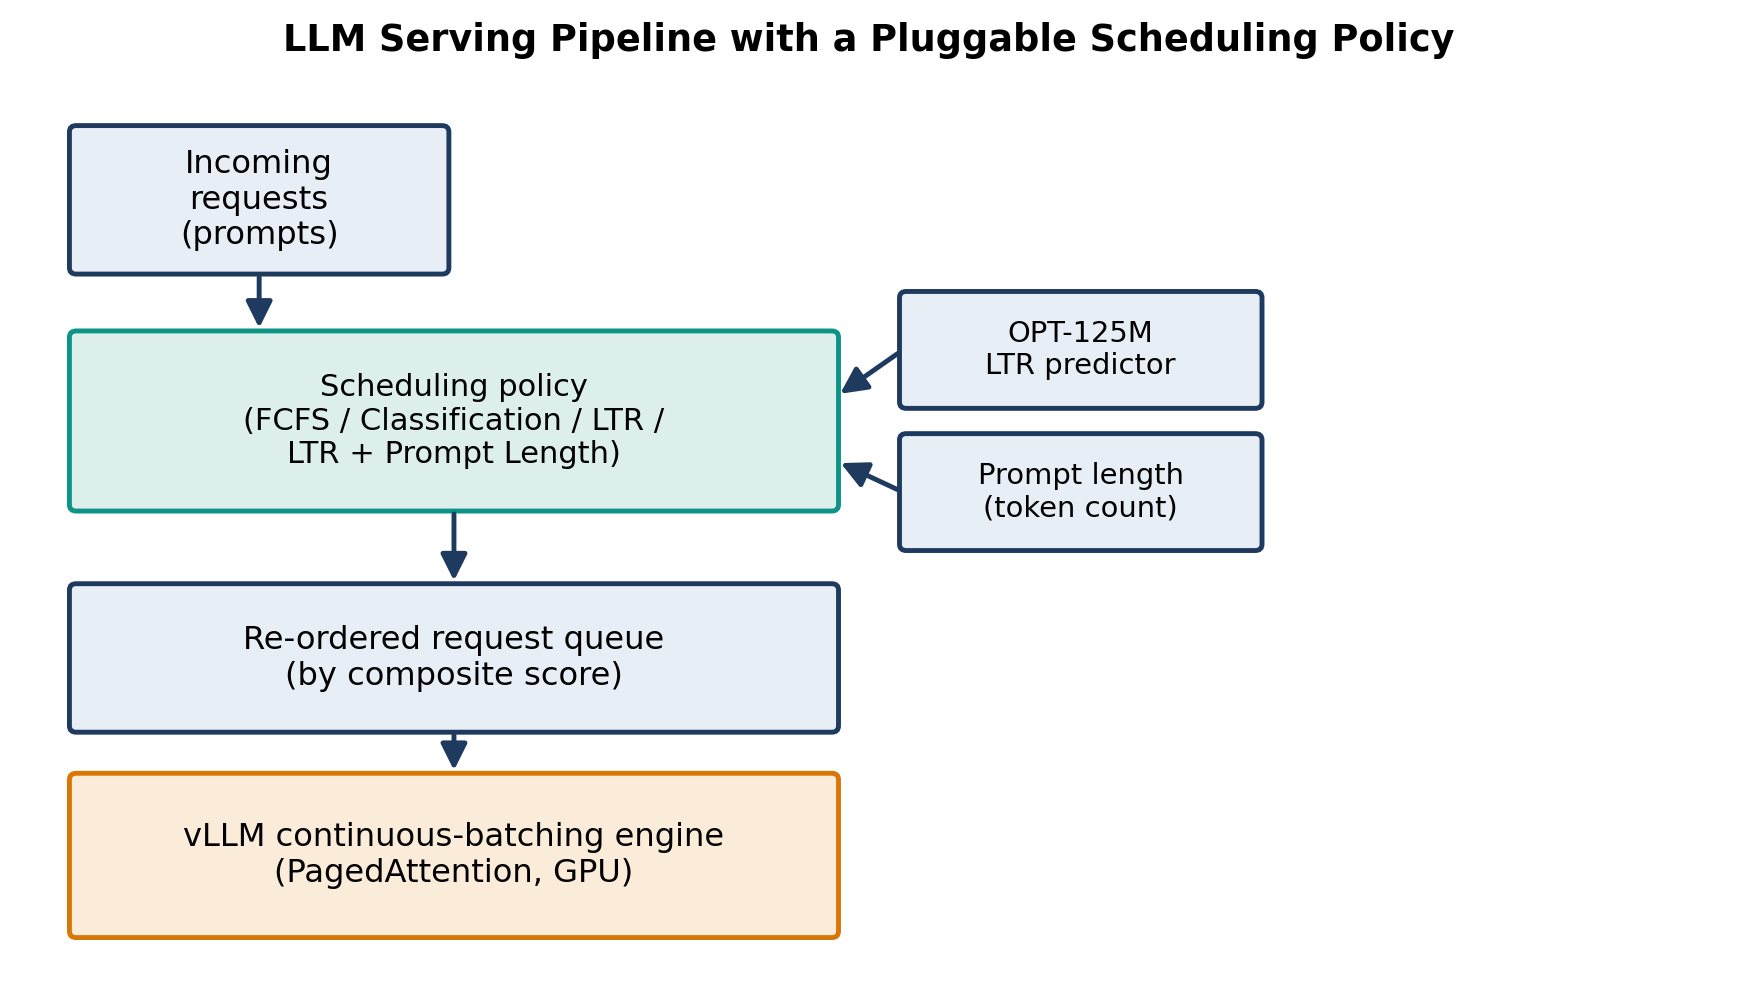
\includegraphics[width=0.95\linewidth]{figures/architecture_pipeline.png}
    \caption{LLM serving pipeline with a pluggable scheduling policy. The
    policy re-orders incoming requests before they are admitted to vLLM's
    continuous-batching engine; the engine itself is unmodified.}
    \label{fig:architecture_pipeline}
\end{figure}

\subsection{Head-of-Line Blocking Under Unknown Output Length}
\label{subsec:hol}

Continuous batching removes idle GPU time between requests, but it does not
by itself protect short requests from being scheduled behind long ones. If
the admission order is FCFS, a request that arrives early but will generate
hundreds of tokens occupies a batch slot for its full decoding duration, and
a request that arrives shortly after but would have finished in a few tokens
must still wait its turn. This is the LLM-serving analogue of HOL blocking:
the request at the head of the queue determines how long everything behind
it waits, regardless of how short that work actually is. Because output
length is not observable before decoding completes, mitigating HOL blocking
requires either estimating it in advance or using a proxy signal that
correlates with it.

\subsection{Learning-to-Rank Scheduling}
\label{subsec:ltr-background}

One way to estimate output length in advance is to train a small model to
predict it, or a value that ranks requests similarly to it, directly from the
prompt text. The LTR approach this work builds on fine-tunes a compact
OPT-125M model~\cite{zhang2022opt} with a ranking loss (ListMLE) so that its
output score orders requests consistently with their true relative output
lengths, rather than predicting the exact token count. Requests are then
admitted in order of this learned score, giving requests expected to be short
priority over requests expected to be long. This is effective to the extent
that the predictor's training distribution matches production traffic, but
the score is the predictor's only signal: if the prompt distribution shifts
or the predictor is uncertain, there is no independent signal to fall back
on. Prompt length is a natural candidate for such a fallback signal, since it
is known instantly and without any additional inference cost;
Figure~\ref{fig:composite_scoring} shows how it is combined with the learned
predictor score to form the composite ranking used in this work, whose
precise formulation is given in Section~\ref{sec:methodology}.

\begin{figure}[t]
    \centering
    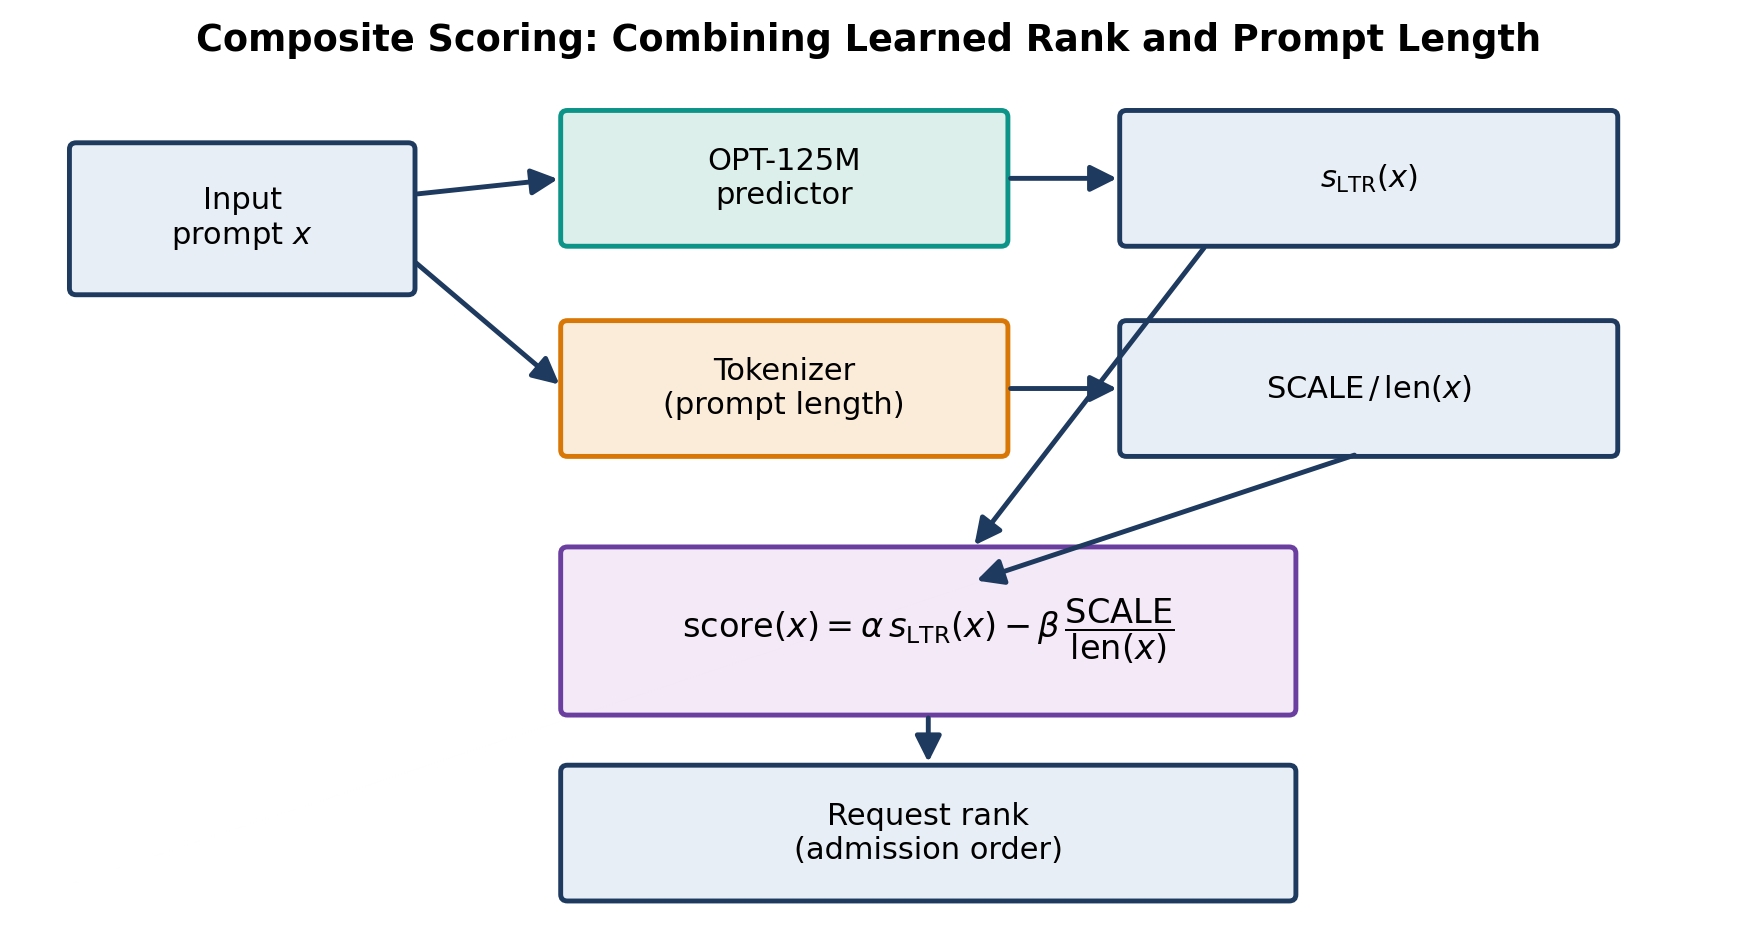
\includegraphics[width=0.95\linewidth]{figures/composite_scoring_architecture.png}
    \caption{Composite scoring architecture. The learned LTR predictor score
    and a normalized prompt-length term are combined into a single ranking
    score used to order the admission queue.}
    \label{fig:composite_scoring}
\end{figure}


\clearpage
\section{Related Work}
\label{sec:related_work}

\subsection{LLM Serving Systems and Memory Management}
\label{subsec:rw-serving}

Orca~\cite{yu2022orca} introduced iteration-level scheduling for
transformer-based generative models, allowing individual requests to enter
and leave a batch between decoding steps rather than waiting for the entire
batch to complete, which is the continuous-batching mechanism this work
depends on. vLLM~\cite{kwon2023vllm} builds on this idea and additionally
introduces PagedAttention, which manages the key-value cache in fixed-size
blocks to reduce memory fragmentation and increase the number of sequences
that can be served concurrently on a fixed amount of GPU memory. Both systems
focus on maximizing GPU utilization and aggregate throughput through
memory-efficient batching; neither prescribes a specific admission-ordering
policy for the requests that populate each batch, which is the aspect of the
serving stack this work targets.

\subsection{Output-Length-Aware and Learning-to-Rank Scheduling}
\label{subsec:rw-scheduling}

A separate line of work argues that batching efficiency alone is insufficient
if the admission order itself causes short requests to wait behind long ones,
and proposes estimating output length ahead of time to inform scheduling.
Response Length Perception and Sequence Scheduling~\cite{zheng2023responselength}
frames this as a classification problem, training a model to bucket prompts
into coarse output-length classes and prioritizing shorter buckets; the
classification-based scheduler evaluated in this paper follows that design.
Efficient LLM Scheduling by Learning to Rank~\cite{fu2024efficient}, the work
this project directly extends, instead trains a compact OPT-125M predictor
with a listwise ranking loss so that its output score orders requests
consistently with their true relative output lengths, without requiring the
predictor to commit to a specific length bucket or exact token count. The
underlying ranking objective follows the learning-to-rank literature more
broadly, including pairwise formulations such as RankNet~\cite{burges2005ranknet}
and listwise formulations such as ListMLE~\cite{xia2008listmle}, the loss used
to train the original predictor in~\cite{fu2024efficient}. This project keeps
that learned predictor intact and asks whether combining its score with an
independent, non-learned signal -- prompt length -- improves robustness when
the predictor's score alone is imperfect, which to our knowledge has not been
examined in prior scheduling work.


\clearpage
\section{Methodology}
\label{sec:methodology}

\subsection{Baseline Framework}

We build on the LTR scheduling framework of~\cite{fu2024efficient}, which
trains an OPT-125M predictor with a ListMLE ranking loss to score prompts by
expected relative output length and uses that score to reorder the admission
queue before requests reach vLLM's generation engine. This ranking step
operates entirely outside vLLM's own continuous-batching scheduler, which
handles the resulting iteration-level batching and memory management
unmodified, as shown in Figure~\ref{fig:architecture_pipeline}.

\subsection{Proposed Extension: Composite Scoring}

Table~\ref{tab:scheduling_policies} summarizes the four scheduling policies
compared in this work. For the proposed extension, each request's admission
priority is
\begin{equation}
    \mathrm{score}(x) = \alpha \, s_{\mathrm{LTR}}(x) \;-\; \beta \, \frac{\mathrm{SCALE}}{\mathrm{len}(x)}
    \label{eq:composite-score}
\end{equation}
where $s_{\mathrm{LTR}}(x)$ is the predictor's learned score for prompt $x$,
$\mathrm{len}(x)$ is its tokenized length, $\mathrm{SCALE}$ brings the length
term onto a comparable numeric range to $s_{\mathrm{LTR}}(x)$, and
$\alpha,\beta$ are fixed weights with $\alpha+\beta=1$. The length term is
subtracted so that longer prompts, absent strong evidence to the contrary
from $s_{\mathrm{LTR}}$, receive a comparatively lower score, reflecting the
assumption that longer prompts more often elicit longer completions.
Requests are admitted in decreasing order of $\mathrm{score}(x)$; since
$\mathrm{len}(x)$ comes directly from tokenization, this signal adds no
inference cost beyond the forward pass already needed for $s_{\mathrm{LTR}}(x)$.

The predictor used for $s_{\mathrm{LTR}}(x)$ in the extension is retrained
with a pairwise margin ranking loss rather than ListMLE, so its score
distribution suits combination with the length term; both share the same
OPT-125M backbone and training set. Table~\ref{tab:hyperparameters} lists the
composite-scoring weights and training hyperparameters used throughout
Section~\ref{sec:evaluation}.

\begin{table}[t]
    \centering
    \caption{Scheduling policies compared in this work.}
    \label{tab:scheduling_policies}
    \begin{tabular}{@{}p{1.5cm}p{5.4cm}@{}}
        \toprule
        Policy & Admission ordering rule \\
        \midrule
        FCFS & Requests admitted in arrival order; no reordering. \\
        Classification & Requests bucketed into coarse predicted output-length classes; shorter buckets prioritized. \\
        LTR & Requests ordered by the OPT-125M predictor's learned ranking score, $s_{\mathrm{LTR}}(x)$, alone. \\
        LTR + Prompt Length (ours) & Requests ordered by the composite score in Eq.~\eqref{eq:composite-score}, combining $s_{\mathrm{LTR}}(x)$ with tokenized prompt length. \\
        \bottomrule
    \end{tabular}
\end{table}

\begin{table}[t]
    \centering
    \caption{Composite scoring and predictor training hyperparameters.}
    \label{tab:hyperparameters}
    \begin{tabular}{@{}ll@{}}
        \toprule
        Parameter & Value \\
        \midrule
        $\alpha$ (LTR score weight) & 0.7 \\
        $\beta$ (prompt-length weight) & 0.3 \\
        SCALE (length-term scale factor) & 100 \\
        Predictor backbone & OPT-125M \\
        Original predictor loss & ListMLE \\
        Extension predictor loss & Pairwise margin \\
        Margin ($m$) & 1.0 \\
        Pair filter threshold ($\delta$) & 0.20 \\
        Training epochs & 10 \\
        \bottomrule
    \end{tabular}
\end{table}


\subsection{Implementation Correction}
\label{subsec:sign-correction}

An early implementation of Eq.~\eqref{eq:composite-score} added the length
term rather than subtracting it, inverting its intended effect. This was
corrected prior to the experiments in Section~\ref{sec:evaluation}; we note
it here for transparency relative to any earlier, uncorrected version of this
codebase.


\clearpage
\section{Evaluation}
\label{sec:evaluation}

\subsection{Experimental Setup}
\label{subsec:setup}

All experiments serve Llama-3.1-8B-Instruct~\cite{dubey2024llama3} in FP16
through vLLM on a single NVIDIA A100 GPU (40GB). Each scheduling policy is
evaluated at seven request arrival rates (5, 10, 20, 30, 40, 50, and 60
requests/second) on each dataset, with requests drawn in a fixed,
pre-computed admission order per policy and submitted to vLLM's offline
\texttt{LLM.generate()} API as a single call, so vLLM's own
continuous-batching scheduler manages iteration-level admission from that
point onward.

\subsection{Datasets}
\label{subsec:datasets}

We use two 1{,}000-request evaluation subsets constructed from the public
LMSYS-Chat-1M conversation dataset~\cite{zheng2023lmsyschat}. Dataset~1 is a
uniform in-distribution sample used to measure baseline scheduling behavior.
Dataset~2 over-samples the extremes of the true output-length distribution to
induce distribution shift between the predictor's training data and its
evaluation data, matching the out-of-distribution stress test used for the
original LTR predictor~\cite{fu2024efficient}. Both subsets are reconstructed
from the public dataset release rather than the original framework's
unpublished 23{,}800-sample file, and should be read as a reconstructed split
rather than an exact reproduction.

\subsection{Scheduling Policies and Metrics}
\label{subsec:policies-metrics}

The four scheduling policies compared are summarized in
Table~\ref{tab:scheduling_policies}. We report: (i) mean throughput in
tokens/second; (ii) two HOL blocking indicators, the ratio of p90 to mean
per-token latency at high load and the slope of mean latency against request
rate, where flatter and lower is better; (iii) time-to-first-token (TTFT),
the delay between arrival and the first generated token, computed from
vLLM's own per-request timestamps rather than approximated from aggregate
batch timing; (iv) peak GPU memory allocation and utilization; and (v)
Kendall's tau~\cite{kendall1938new} between each score and true output
length.

\subsection{Throughput}
\label{subsec:results-throughput}

Table~\ref{tab:throughput} reports mean throughput for each scheduler.
LTR + Prompt Length achieves the highest throughput of the four policies on
both datasets, improving over the original LTR scheduler by approximately
31.7\% on Dataset~1 and 6.7\% on Dataset~2. Notably, the original LTR and
Classification schedulers both under-perform plain FCFS on Dataset~1 despite
their explicit goal of reducing HOL blocking, suggesting that a miscalibrated
or overly aggressive reordering can trade away throughput even as it changes
tail-latency behavior; the composite score's use of prompt length as a
stabilizing signal appears to avoid this failure mode on the datasets tested.

\begin{figure*}[t]
    \centering
    \begin{subfigure}[b]{0.48\textwidth}
        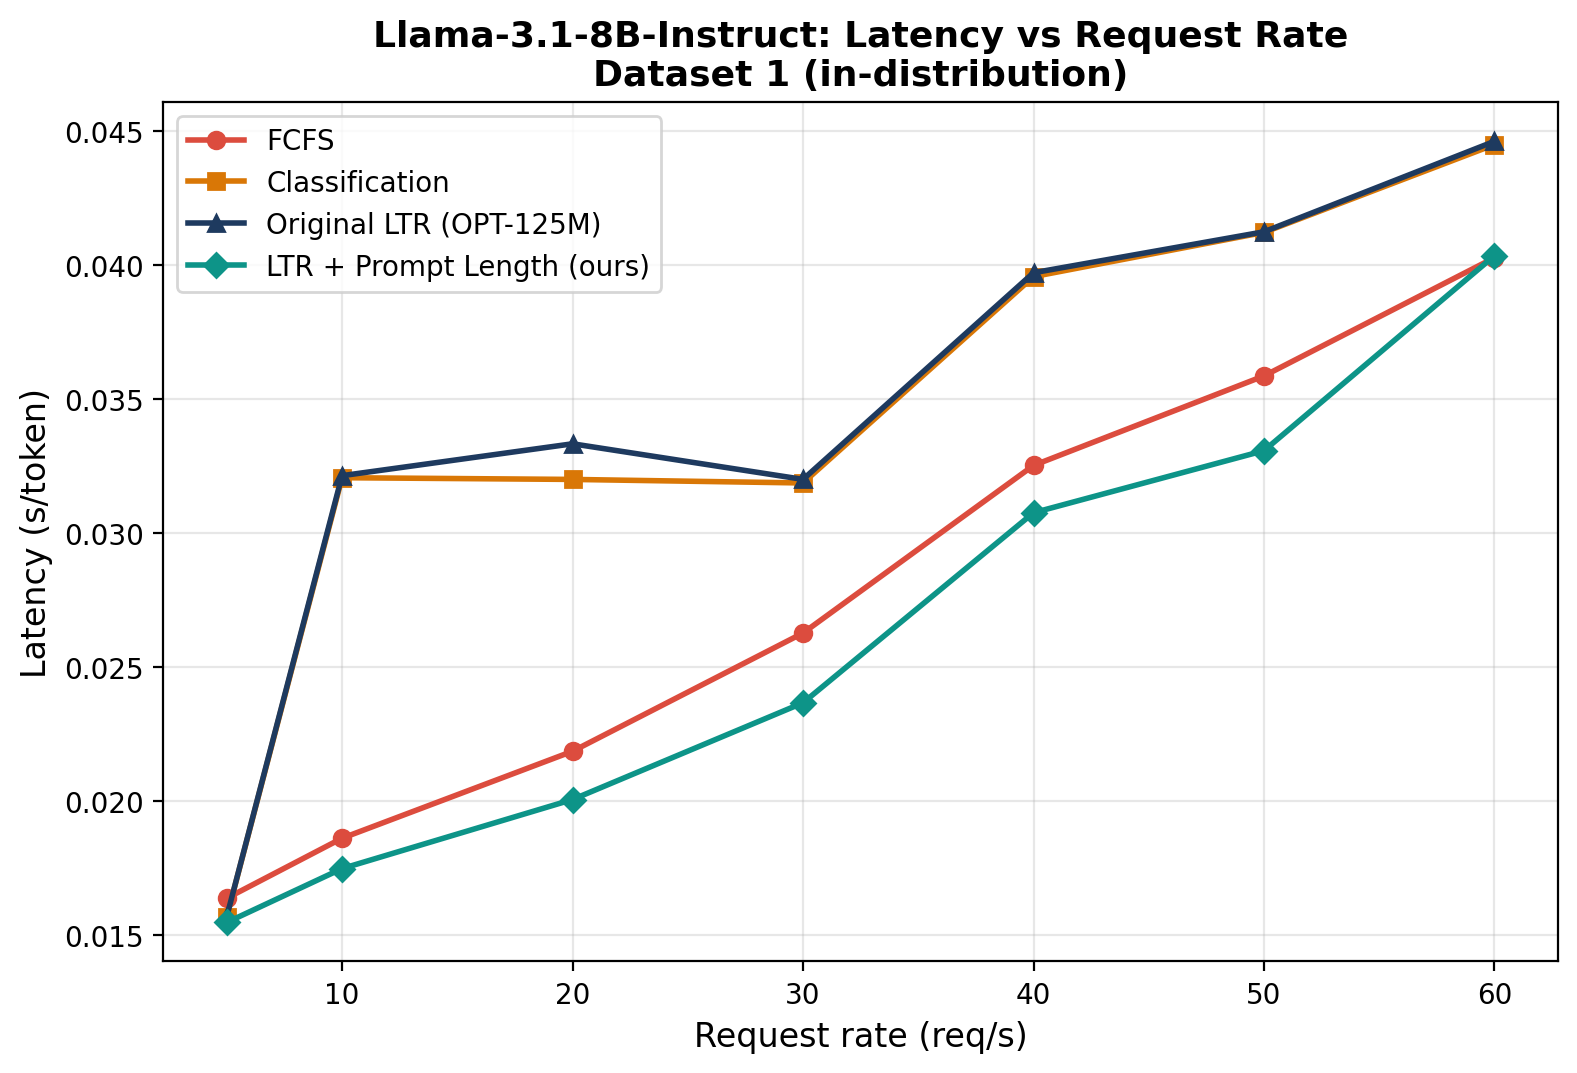
\includegraphics[width=\linewidth,height=3.5cm,keepaspectratio]{figures/latency_dataset1.png}
        \caption{Dataset 1 (in-distribution)}
        \label{fig:latency-d1}
    \end{subfigure}
    \hfill
    \begin{subfigure}[b]{0.48\textwidth}
        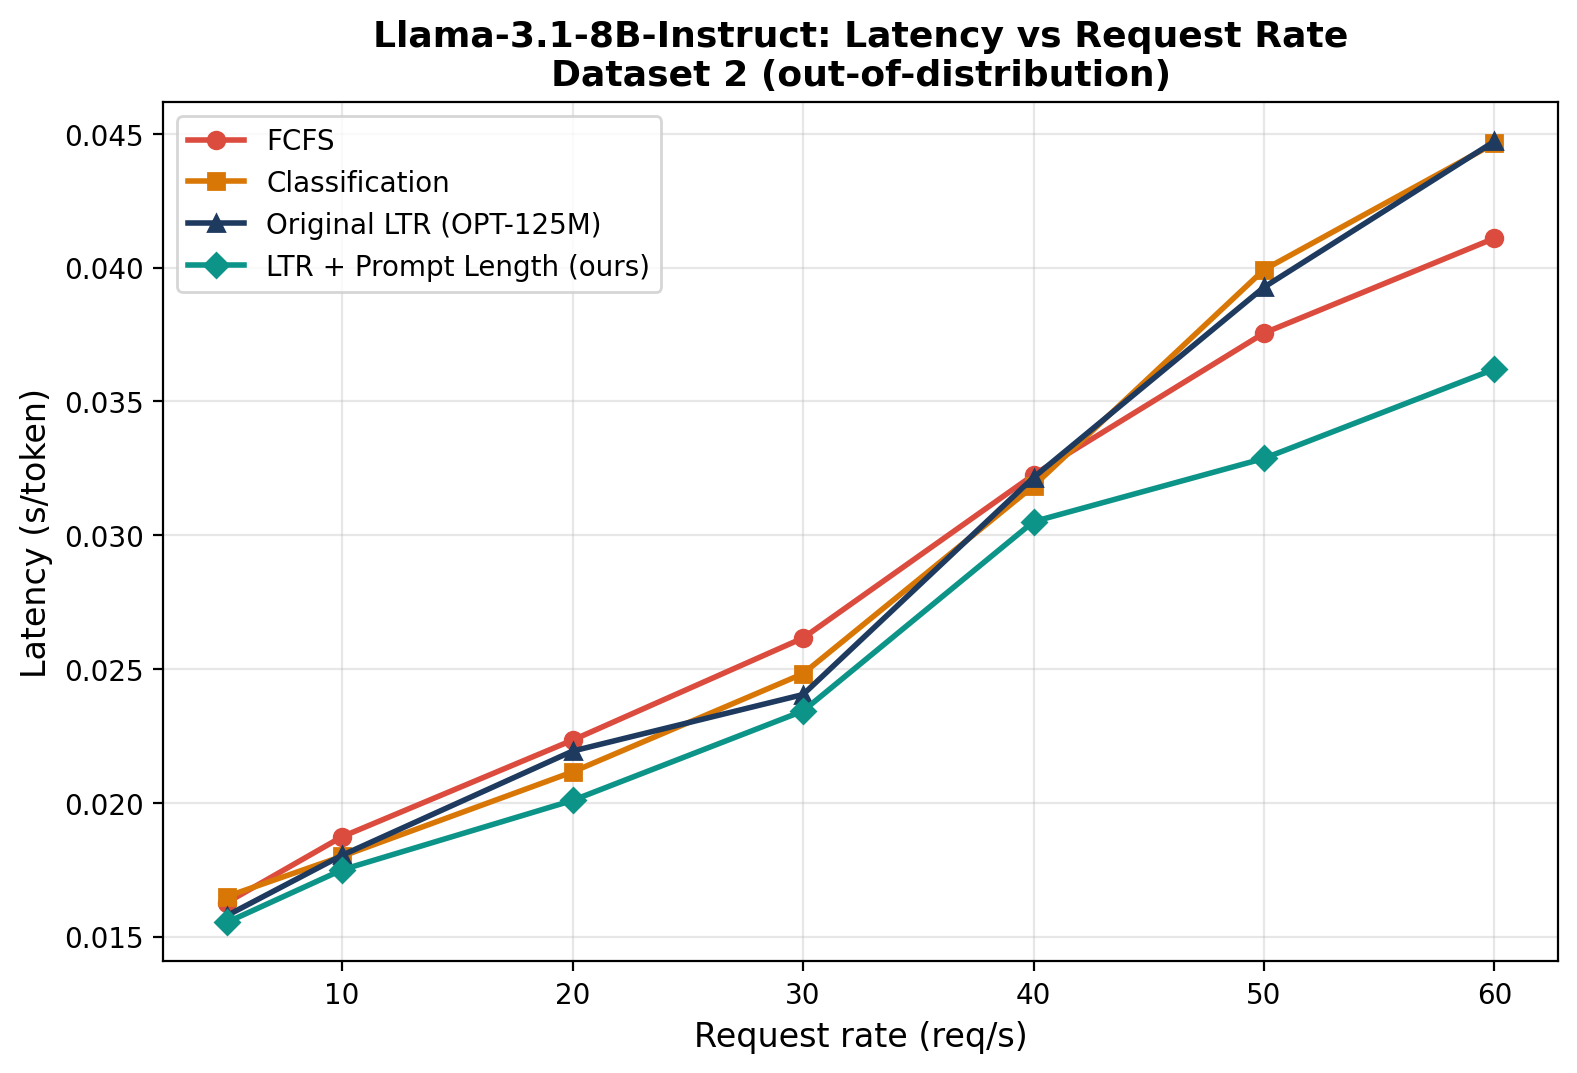
\includegraphics[width=\linewidth,height=3.5cm,keepaspectratio]{figures/latency_dataset2.png}
        \caption{Dataset 2 (out-of-distribution)}
        \label{fig:latency-d2}
    \end{subfigure}
    \caption{Mean per-token latency versus request rate, by scheduler.}
    \label{fig:latency-vs-rate}
\end{figure*}

\subsection{Latency Versus Request Rate}
\label{subsec:results-latency}

Figure~\ref{fig:latency-vs-rate} shows mean per-token latency as request rate
increases from 5 to 60 requests/second. All four policies show latency
rising with request rate, as expected once arrival rate approaches the GPU's
sustainable throughput, but the rate of increase differs by policy;
Table~\ref{tab:hol_blocking} quantifies this as the latency-vs-rate slope,
discussed in Section~\ref{subsec:results-hol}.

\subsection{Time-to-First-Token}
\label{subsec:results-ttft}

Figure~\ref{fig:ttft-vs-rate} reports mean and p90 TTFT across the same
sweep. At the highest tested rate (60 req/s), mean TTFT for LTR + Prompt
Length is 0.157s, versus 1.034s for FCFS, 0.594s for Classification, and
0.600s for the original LTR scheduler; p90 TTFT is 0.288s versus 1.825s for
FCFS. Because TTFT is not normalized by a request's output length, this gap
is a more direct indication of reduced HOL blocking than the per-token
latency metrics in Section~\ref{subsec:results-latency} alone.

\begin{figure*}[t]
    \centering
    \begin{subfigure}[b]{0.48\textwidth}
        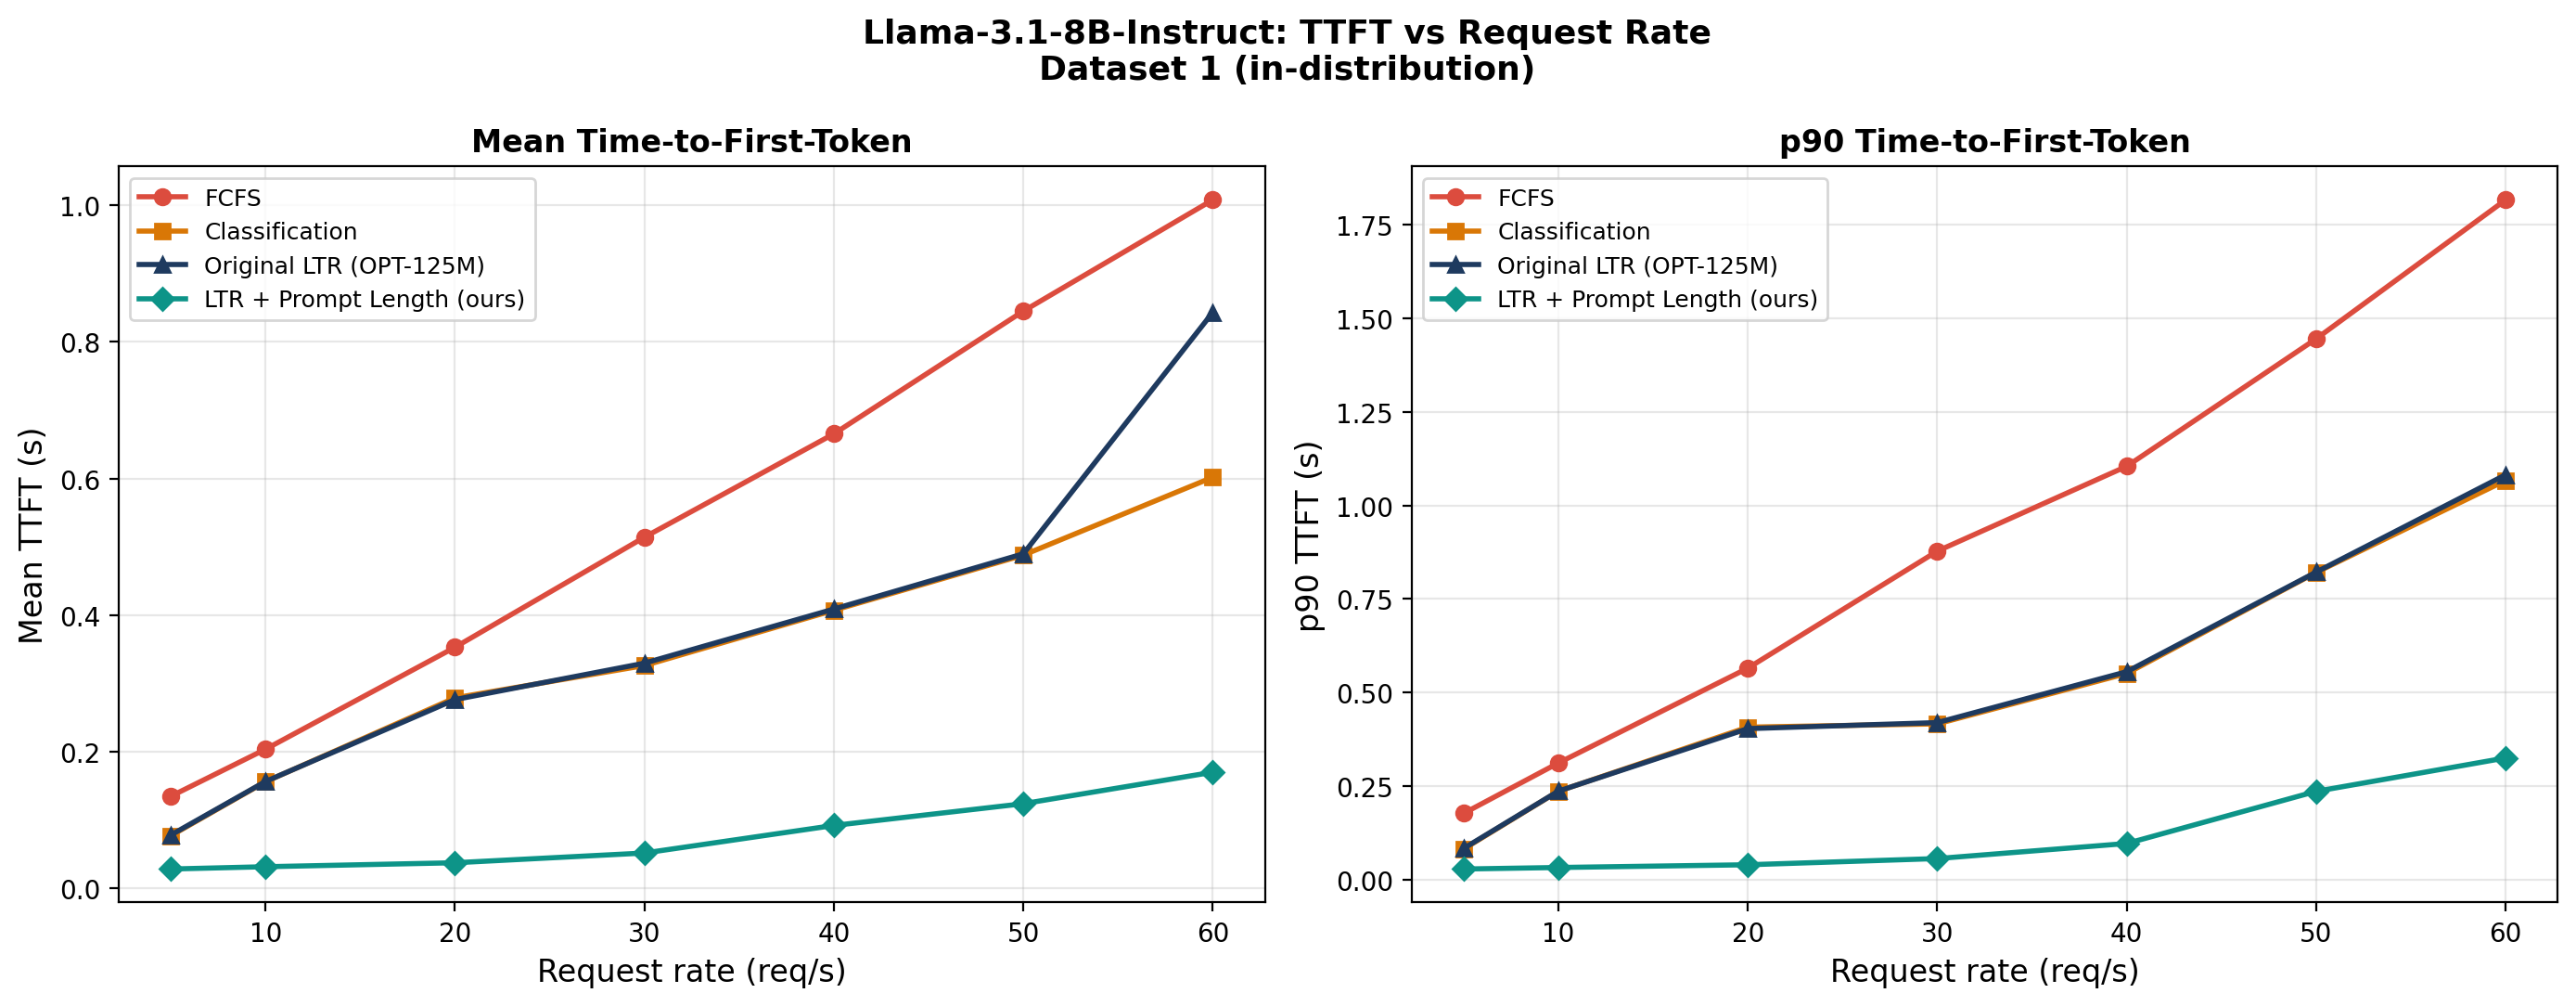
\includegraphics[width=\linewidth,height=3.5cm,keepaspectratio]{figures/ttft_dataset1.png}
        \caption{Dataset 1 (in-distribution)}
        \label{fig:ttft-d1}
    \end{subfigure}
    \hfill
    \begin{subfigure}[b]{0.48\textwidth}
        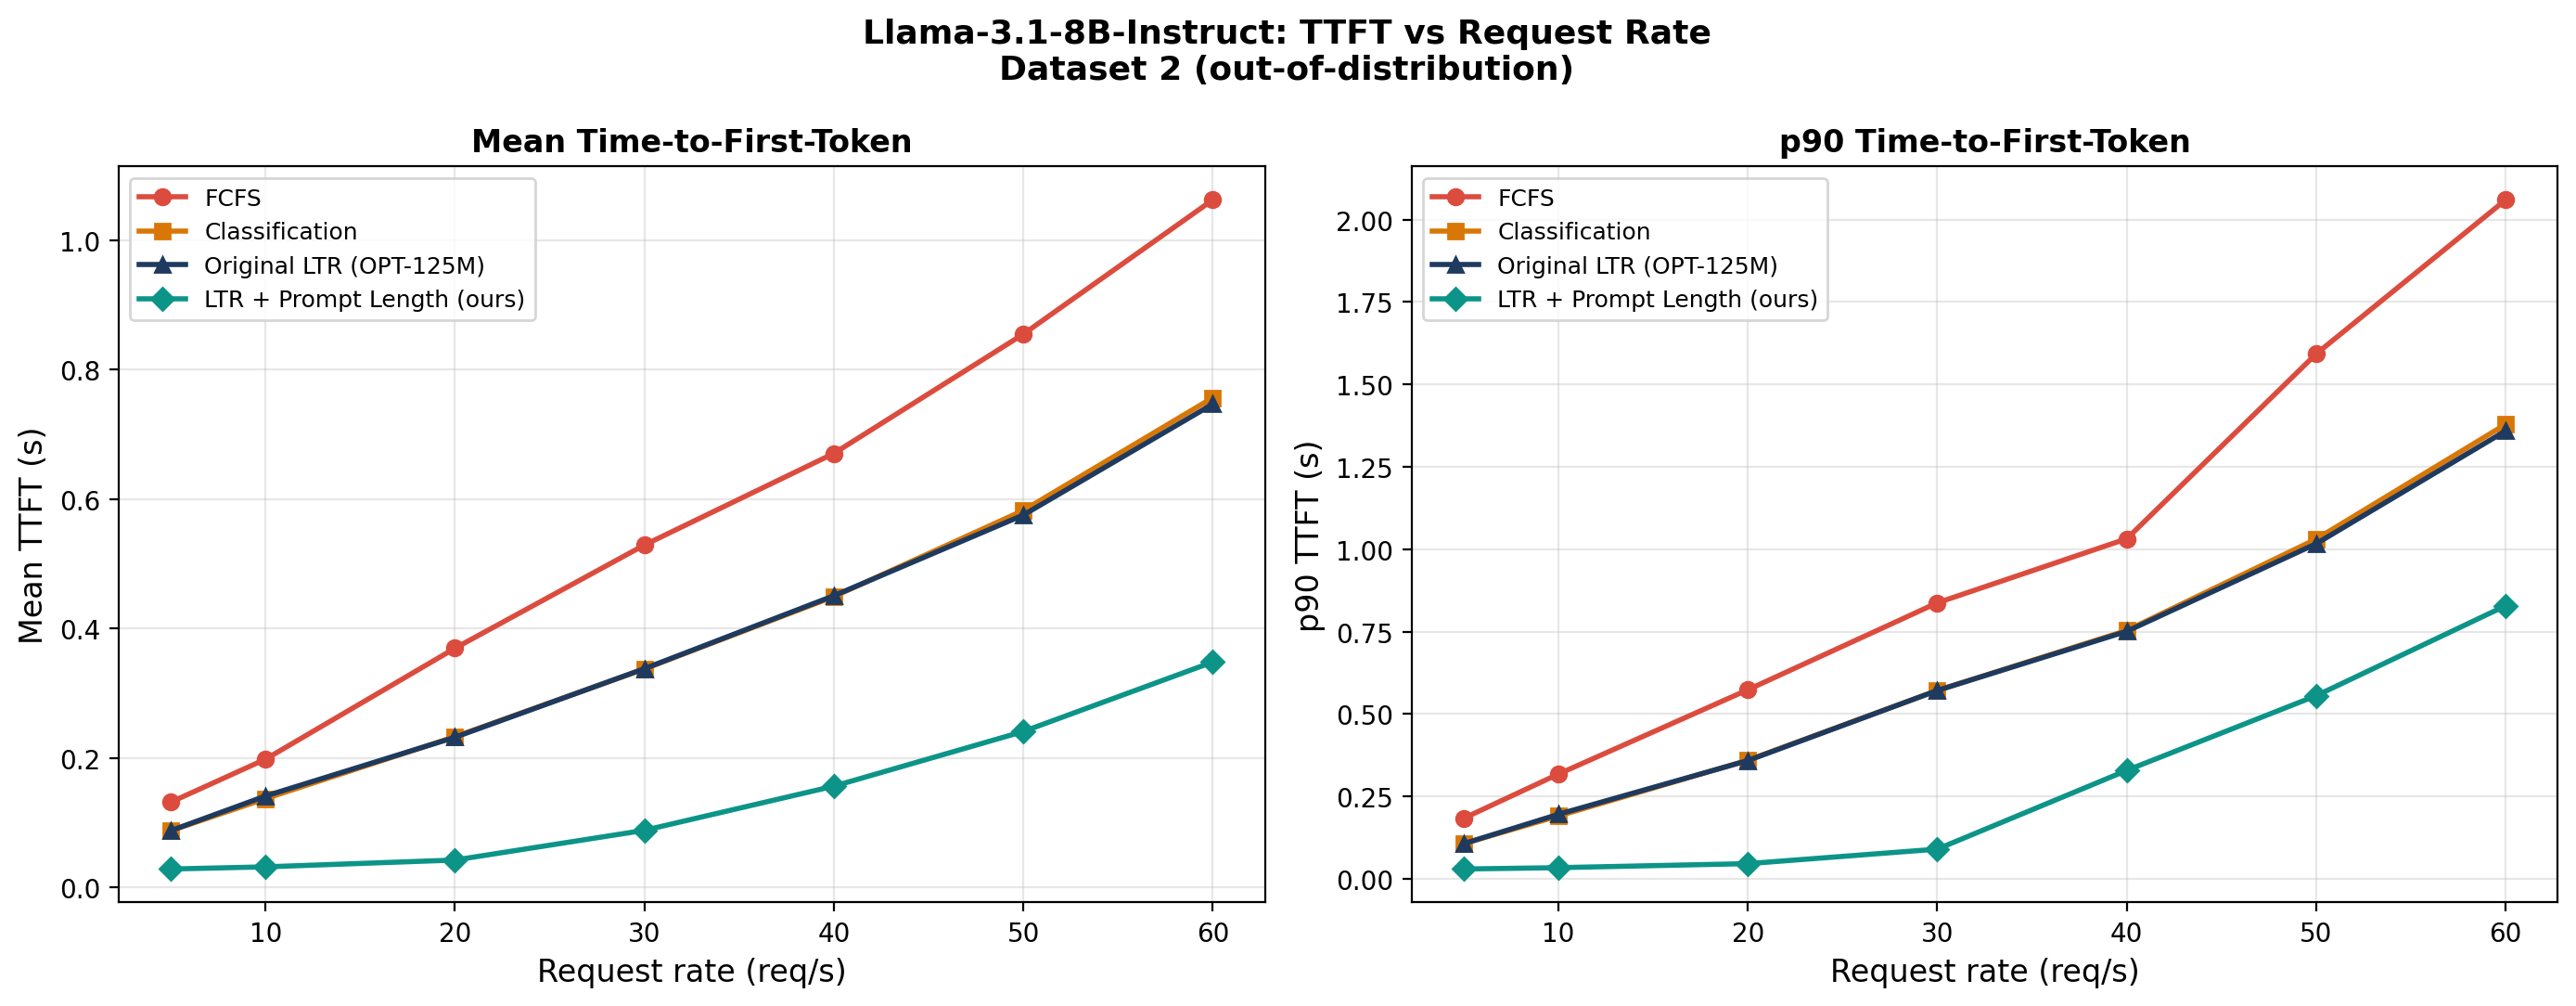
\includegraphics[width=\linewidth,height=3.5cm,keepaspectratio]{figures/ttft_dataset2.png}
        \caption{Dataset 2 (out-of-distribution)}
        \label{fig:ttft-d2}
    \end{subfigure}
    \caption{Mean and p90 time-to-first-token versus request rate, by
    scheduler.}
    \label{fig:ttft-vs-rate}
\end{figure*}

\subsection{Head-of-Line Blocking Indicators}
\label{subsec:results-hol}

Table~\ref{tab:hol_blocking} and Figure~\ref{fig:hol-blocking} summarize the
p90/mean latency ratio at high load and the latency-vs-rate slope. The
Classification and original LTR schedulers achieve the lowest p90/mean ratio
on Dataset~1, indicating that an accurate length estimate compresses tail
latency effectively; however, both show a steeper latency-vs-rate slope than
FCFS on Dataset~1, meaning latency degrades faster under load. LTR + Prompt
Length achieves the lowest slope on Dataset~2 (OOD) among all four policies,
consistent with the prompt-length signal stabilizing the ranking precisely
when the learned predictor is out of distribution.

\begin{figure*}[t]
    \centering
    \begin{subfigure}[b]{0.48\textwidth}
        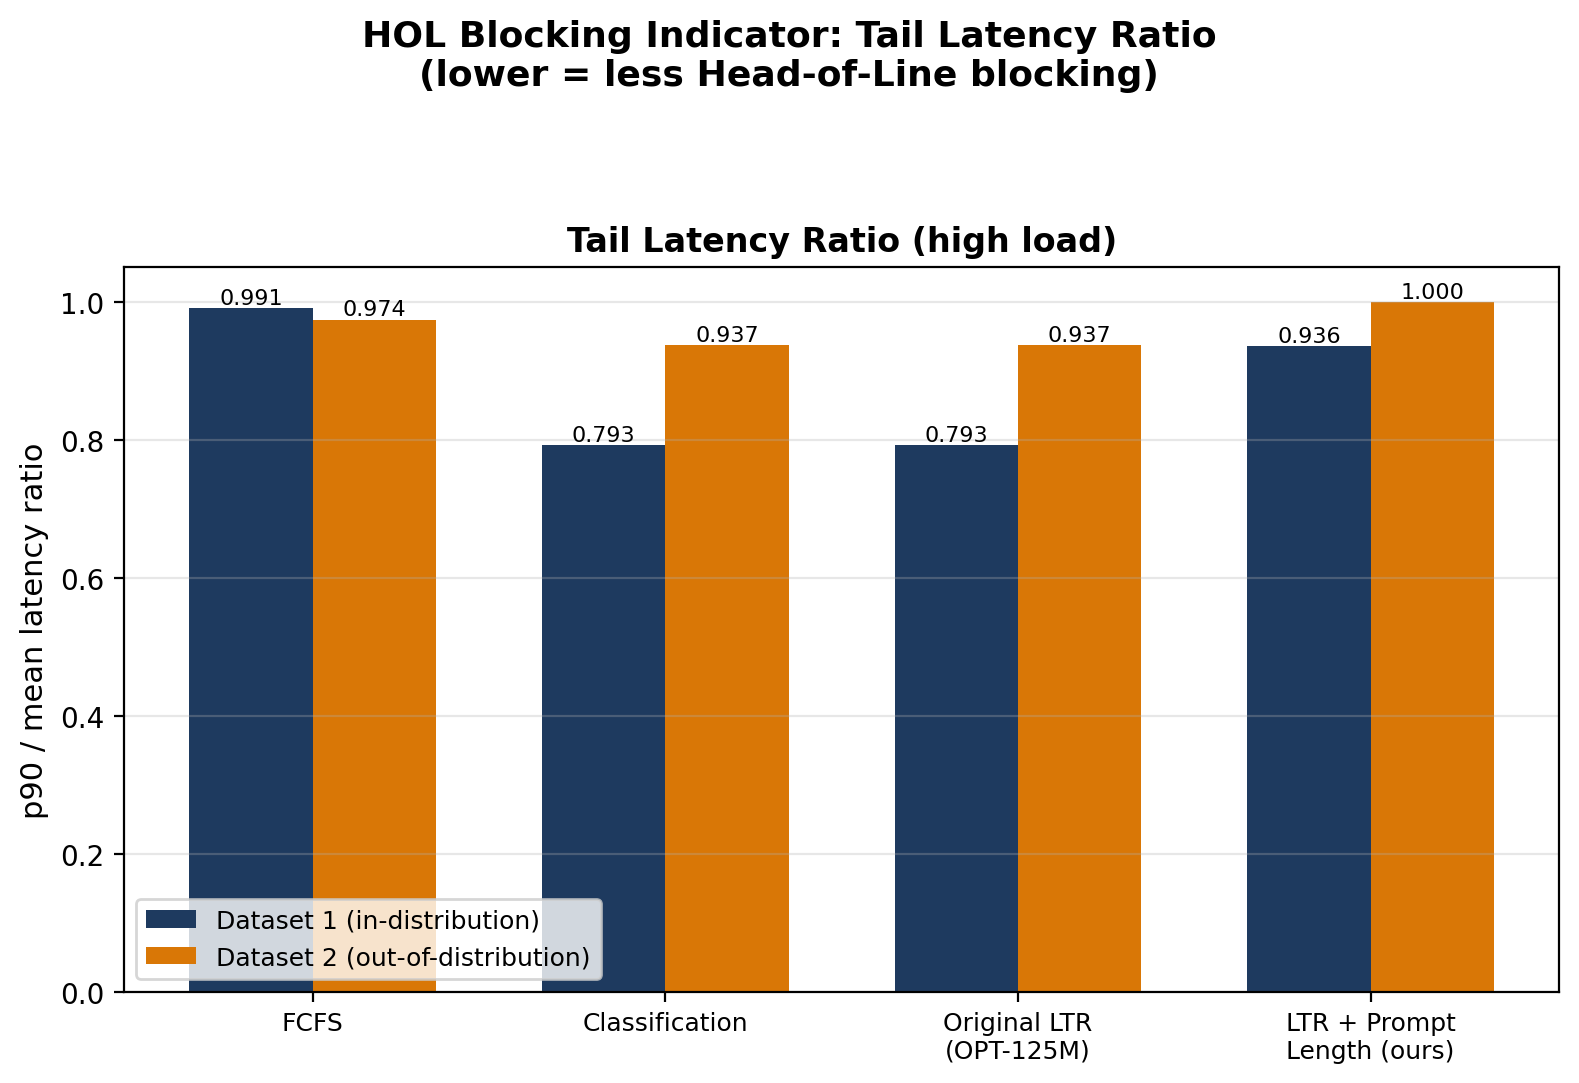
\includegraphics[width=\linewidth,height=3.5cm,keepaspectratio]{figures/hol_blocking_ratio.png}
        \caption{p90/mean latency ratio at high load}
        \label{fig:hol-ratio}
    \end{subfigure}
    \hfill
    \begin{subfigure}[b]{0.48\textwidth}
        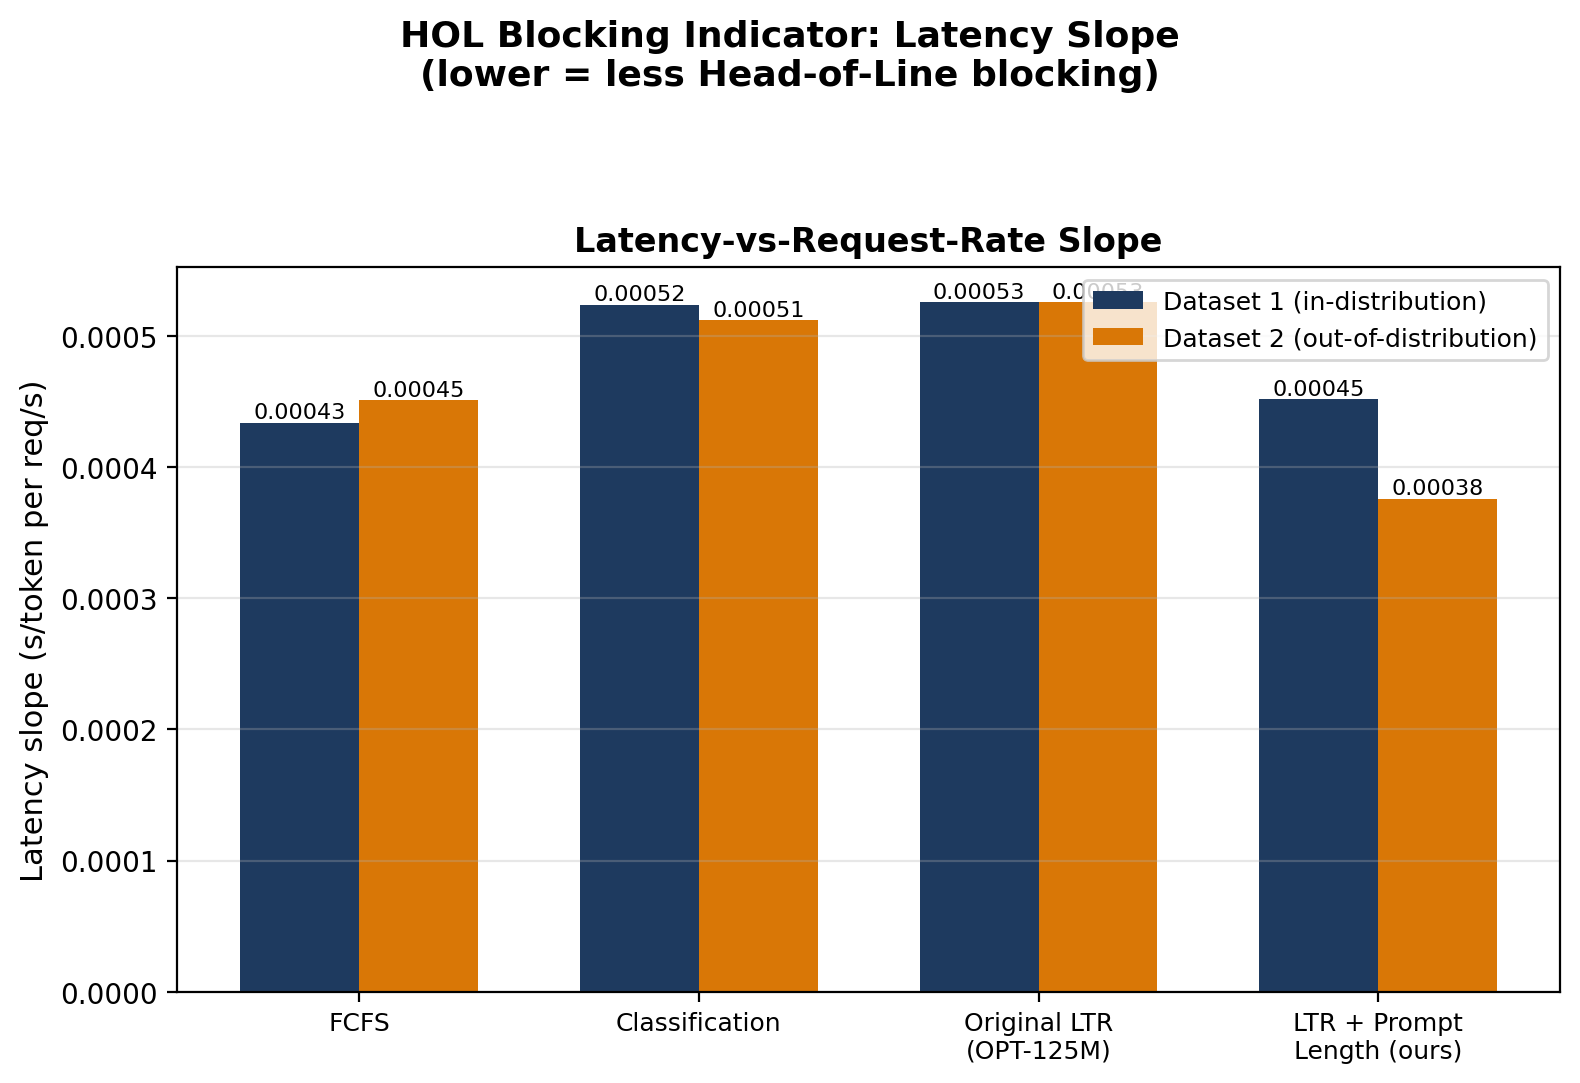
\includegraphics[width=\linewidth,height=3.5cm,keepaspectratio]{figures/hol_blocking_slope.png}
        \caption{Latency-vs-request-rate slope}
        \label{fig:hol-slope}
    \end{subfigure}
    \caption{HOL blocking indicators by scheduler and dataset.}
    \label{fig:hol-blocking}
\end{figure*}

\subsection{GPU Resource Utilization}
\label{subsec:results-gpu}

Table~\ref{tab:gpu_utilization} and Figure~\ref{fig:gpu-utilization} report
peak GPU memory allocation and utilization while serving each dataset.
Utilization stays above 86\% of the profiled budget on both datasets,
indicating the reordering step adds no meaningful memory overhead, since it
operates only on tokenized prompt lengths and predictor scores.

\begin{figure}[t]
    \centering
    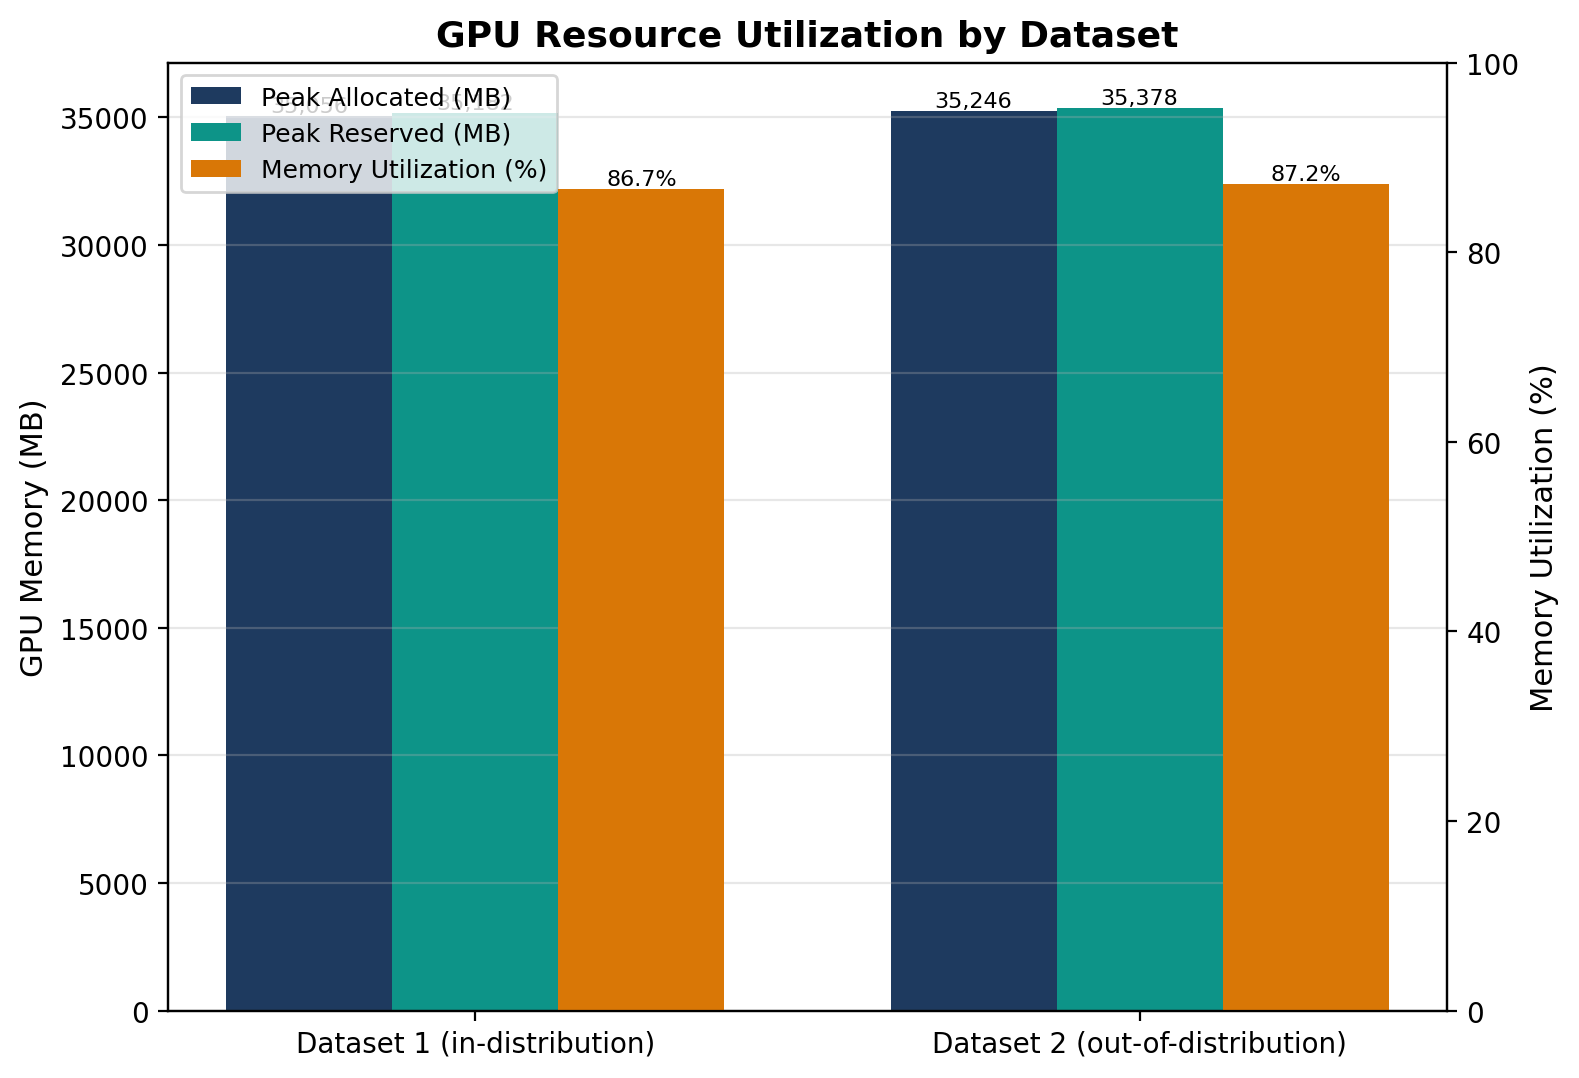
\includegraphics[width=0.8\linewidth,height=4.2cm,keepaspectratio]{figures/gpu_utilization.png}
    \caption{Peak GPU memory allocation, peak reserved memory, and memory
    utilization by dataset.}
    \label{fig:gpu-utilization}
\end{figure}

\subsection{Ranking Quality: Kendall's Tau}
\label{subsec:results-tau}

Table~\ref{tab:kendalls_tau} reports Kendall's tau between each score and
true output length on the Dataset~2 (OOD) held-out set. The composite score
modestly improves over the LTR-only score (0.3445 to 0.3457,
$\Delta=+0.0011$), indicating the prompt-length signal does not degrade
ranking quality under distribution shift.

\begin{table}[t]
    \centering
    \small
    \caption{Mean throughput (tokens/s) by scheduler.}
    \label{tab:throughput}
    \begin{tabular}{@{}lcc@{}}
        \toprule
        Scheduler & D1 (in-dist.) & D2 (OOD) \\
        \midrule
        FCFS                & 40.47 & 40.06 \\
        Classification      & 32.86 & 41.22 \\
        LTR                 & 32.80 & 41.06 \\
        LTR+PL (ours)       & \textbf{43.21} & \textbf{43.82} \\
        \bottomrule
    \end{tabular}
\end{table}

\begin{table*}[t]
    \centering
    \caption{HOL blocking indicators by scheduler: p90/mean latency ratio at
    high load (lower is better) and latency-vs-request-rate slope in
    seconds/token per req/s (lower is better).}
    \label{tab:hol_blocking}
    \begin{tabular}{@{}lcccc@{}}
        \toprule
        & \multicolumn{2}{c}{p90/mean ratio} & \multicolumn{2}{c}{Slope ($\times 10^{-4}$)} \\
        Scheduler & D1 & D2 & D1 & D2 \\
        \midrule
        FCFS                        & 0.991 & 0.974 & 4.3 & 4.7 \\
        Classification              & 0.793 & 0.937 & 5.3 & 5.2 \\
        LTR                         & 0.793 & 0.937 & 5.2 & 5.2 \\
        LTR + Prompt Length (ours)  & 0.936 & 1.000 & 4.5 & 3.8 \\
        \bottomrule
    \end{tabular}
\end{table*}

\begin{table}[t]
    \centering
    \small
    \caption{GPU resource utilization on a single NVIDIA A100 (40GB, FP16).}
    \label{tab:gpu_utilization}
    \begin{tabular}{@{}lcc@{}}
        \toprule
        Dataset & Peak alloc. (MB) & Mem. util. \\
        \midrule
        D1 (in-dist.) & 35{,}055.6 & 86.7\% \\
        D2 (OOD)      & 35{,}246.4 & 87.2\% \\
        \bottomrule
    \end{tabular}
\end{table}

\begin{table}[t]
    \centering
    \caption{Kendall's tau ranking quality against true output length,
    evaluated on the Dataset 2 (out-of-distribution) held-out set
    ($n=1{,}000$, $\alpha=0.7$, $\beta=0.3$).}
    \label{tab:kendalls_tau}
    \begin{tabular}{@{}lc@{}}
        \toprule
        Score & Kendall's $\tau$ \\
        \midrule
        LTR only                   & 0.3445 \\
        LTR + Prompt Length (ours) & 0.3457 \\
        \midrule
        $\Delta$                   & $+0.0011$ \\
        \bottomrule
    \end{tabular}
\end{table}



\clearpage
\section{Discussion}
\label{sec:discussion}

The results in Section~\ref{sec:evaluation} suggest that a cheap, non-learned
signal can meaningfully complement a learned ranking score rather than merely
duplicate it. Prompt length costs nothing beyond tokenization, is always
available regardless of how confident or well-calibrated the LTR predictor
is, and, unlike the predictor's score, cannot itself be affected by
distribution shift in the prompt distribution. This likely explains why the
composite scheduler's advantage over the LTR-only scheduler is more
pronounced on the out-of-distribution dataset than on the in-distribution
one: the length signal has the most to contribute exactly when the learned
score is least reliable.

\subsection{Limitations}
\label{subsec:limitations}

Several limitations qualify these findings. First, prompts in this evaluation
were submitted to the serving model without applying its chat template; we
verified in earlier diagnostic runs that this caused a substantial fraction of
generations to reach the configured maximum token cap rather than terminate
naturally, which compresses the observed spread of true output lengths and
should be considered when interpreting the absolute latency and HOL-blocking
values reported here. Second, the composite weights $\alpha$ and $\beta$ in
Eq.~\eqref{eq:composite-score} were fixed manually rather than learned or
tuned per dataset, so the reported results reflect one operating point rather
than the best achievable trade-off. Third, all scheduling policies in this
evaluation compute an admission order over the entire batch of requests
before submission, rather than reordering a continuously arriving stream in
real time; this differs from FCFS, which processes requests as they truly
arrive, and is a potential confound when comparing tail-latency behavior
across policies. Fourth, the evaluation is limited to a single model
(Llama-3.1-8B-Instruct), a single GPU (one NVIDIA A100), and two
1{,}000-request held-out sets, which may not capture the full range of
production traffic patterns or hardware configurations. Finally, the serving
environment uses a newer vLLM release (0.6.1.post2) than the original LTR
framework's target version (0.4.1), a substitution required because the
original version has no prebuilt wheel for the Python 3.12 environment used
here and because the platform's pre-installed PyTorch build is not
ABI-compatible with vLLM's compiled CUDA extensions; this limits direct
numerical comparison to results reported under the original framework's
software stack.

\subsection{Future Work}
\label{subsec:future-work}

Over the next six months, we intend to: (1) rerun the full benchmark suite
with the model's chat template correctly applied, to obtain output-length
distributions and latency figures free of the max-token-cap artifact
described above; (2) replace the fixed $\alpha, \beta$ weighting with a
learned or validation-tuned combination, potentially conditioned on the
predictor's own confidence; (3) evaluate the composite scheduler under a
true streaming arrival process rather than a pre-sorted batch, to remove the
admission-order confound noted above; (4) extend the evaluation to
additional model sizes and a multi-GPU, tensor-parallel serving
configuration; and (5) investigate using time-to-first-token directly as a
scheduling objective, rather than only as an evaluation metric, given its
sensitivity to queuing delay observed in Section~\ref{subsec:results-ttft}.


\clearpage
\section{Conclusion}
\label{sec:conclusion}

This paper presented a composite scheduling score that augments a learned
LTR predictor with tokenized prompt length as a lightweight, always-available
secondary signal, and integrated it into vLLM alongside FCFS, a
classification-based baseline, and the original LTR scheduler. Across two
1{,}000-request LMSYS-Chat-1M subsets served with Llama-3.1-8B-Instruct on a
single A100 GPU, the composite scheduler achieved the highest mean throughput
of the four policies on both datasets, reduced time-to-first-token
substantially at high request rates, and modestly improved ranking quality
under distribution shift. These results suggest that combining a learned
ranking signal with an inexpensive, non-learned one is a practical way to make
output-length-aware LLM scheduling more robust, and the limitations discussed
in Section~\ref{sec:discussion} outline the concrete steps needed to
strengthen this evaluation further.


\clearpage
\appendices
\section{}
\label{sec:appendix}

% Per assignment instructions, this section contains only the screenshot of
% the GitHub latex_source/ directory listing, after it has been pushed to
% the repository -- no accompanying text.
%
% TODO: replace figures/appendix_latex_source_screenshot.png with an actual
% screenshot of https://github.com/waizinmon/prompt-aware-ltr/tree/main/latex_source
% taken after pushing this latex_source/ directory to GitHub.

\vspace*{\fill}
\begin{center}
    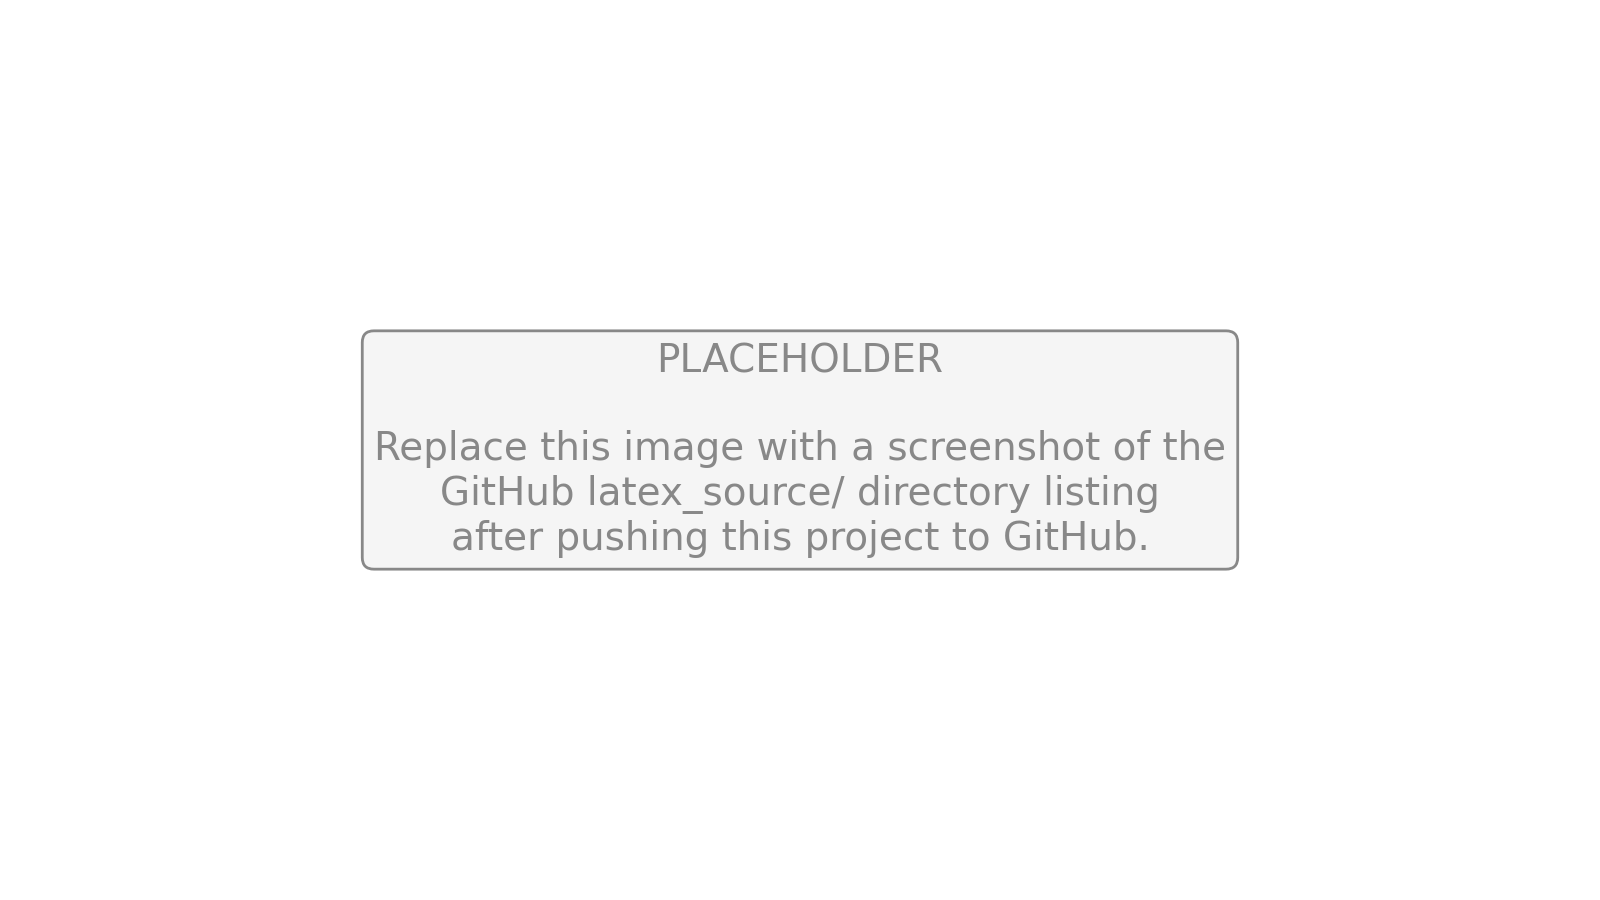
\includegraphics[width=0.85\linewidth]{figures/appendix_latex_source_screenshot.png}
\end{center}
\vspace*{\fill}


\clearpage
\label{sec:references}
\bibliographystyle{IEEEtran}
\bibliography{refs}

\end{document}
